This paper reports on an exploratory survey of 797 engineers at Microsoft examining the relationship between personality traits, work practices, and professional beliefs. Using the Five-Factor Model (Openness, Conscientiousness, Extraversion, Agreeableness, and Neuroticism) and statistical analyses including Kruskal–Wallis tests with multiple-hypothesis correction, the authors analyzed differences across roles, practices, and viewpoints.

The results reveal relatively few strong personality differences. No significant differences were found between developers and testers, while managers were more conscientious and extraverted. Engineers who built their own tools were more open, conscientious, and extraverted, and less neurotic. Agreement with statements such as “Agile development is awesome” was also associated with higher extraversion and lower neuroticism. Overall, the findings suggest that personality differences among software engineers exist but are limited in scope.

\section{Motivation}
There has been sustained interest in understanding what makes effective and successful software engineers, particularly as software development has become increasingly collaborative and complex. Prior research has explored the characteristics of high-performing engineers and the broader question of what differentiates great software professionals from their peers \cite{Li2015}. At the same time, a substantial body of work has investigated the role of personality in software engineering, examining how individual traits relate to job satisfaction, software quality, team effectiveness, and project outcomes \cite{Cruz2015,Capretz2003}. These studies suggest that personality traits may influence not only individual performance but also team dynamics and the overall success of software projects \cite{CapretzAhmed2010}.

Despite decades of research, empirical evidence remains fragmented, and findings are sometimes inconsistent. For example, prior studies have reported personality differences across software roles such as developers and testers \cite{Kanij2015}, yet these findings have not been broadly validated in large industrial contexts. Moreover, much of the existing work has focused on personality in relation to performance or team composition, rather than examining how personality relates to engineers’ everyday work practices and beliefs about controversial or widely debated development practices. Understanding these relationships is important because beliefs about methodologies, tooling, and development practices shape engineering decisions, team culture, and adoption of processes. Therefore, the paper is motivated by the need to systematically examine, within a large industrial setting, how personality traits relate to engineers’ work practices and beliefs, and whether personality meaningfully differentiates subgroups within the software engineering population.

\section{Methodology}
The study employed a survey-based empirical methodology to investigate the relationship between software engineers’ personality traits, work practices, and professional beliefs. The research was conducted within a large industrial organization and targeted engineers in the United States. A total of 3,000 engineers were invited to participate in an anonymous online survey, and 797 responses were received, corresponding to a 26\% response rate. The survey was advertised as a “Developer Personality Survey,” and participation was voluntary. To encourage participation, the invitation was personalized, anonymity was preserved, and respondents were offered entry into a gift-card drawing via a separate communication channel to maintain confidentiality .

The survey instrument consisted of two main components: a personality assessment and a set of non-personality questions addressing demographics, work practices, and beliefs. Personality was measured using the International Personality Item Pool (IPIP), a widely used public-domain instrument aligned with the Five-Factor Model\footnotemark[1] (FFM) of personality \cite{Goldberg2006}. The Five-Factor Model—often referred to as the OCEAN model—comprises five dimensions:

\begin{itemize}
    \item Openness to experience,
    \item Conscientiousness,
    \item Extraversion,
    \item Agreeableness,
    \item Neuroticism.
\end{itemize}

\footnotetext[1]{The authors selected the Five-Factor Model rather than the Myers–Briggs Type Indicator (MBTI) due to its stronger theoretical grounding, higher empirical validity, and superior test–retest reliability \cite{CostaMcCrae1992,Pittenger1993}.}
The personality assessment included 50 IPIP items. Only engineers based in the United States were surveyed to minimize cultural and linguistic ambiguity in interpreting survey items, particularly those containing idiomatic expressions .

Following the personality inventory, participants answered 23 additional multiple-choice questions categorized as follows:

\begin{itemize}
    \item 3 demographic questions (e.g., role, management status, educational background),
    \item 12 work-practice questions (e.g., tool usage, remote work, coding habits),
    \item 8 belief-related questions (e.g., opinions on Agile, code reviews, static vs.\ dynamic typing).
\end{itemize}

Belief questions were derived in part from controversial programming discussions, with the intention of capturing variation in strongly held professional viewpoints. All non-personality items were structured as categorical responses (e.g., Yes/No or Disagree/Neutral/Agree).

The data analysis proceeded in two stages. First, descriptive statistics were computed to examine the distributions of responses to all non-personality questions. This step provided an overview of the demographic composition, work-practice patterns, and diversity of beliefs within the sample .

Second, inferential statistical analysis was conducted to identify relationships between personality traits and responses to non-personality questions. Because several survey questions contained more than two response categories, the authors employed the Kruskal–Wallis rank-sum test to evaluate differences in personality scores across groups. For each of the 23 non-personality questions, five separate tests were conducted—one for each personality dimension—resulting in 115 hypothesis tests in total.

To enable comparison across groups, personality scores were normalized such that the mean was set to 25 and the standard deviation to 5, following established normalization practices in cross-population personality research \cite{Schmitt2007}. Higher scores indicate stronger expression of the respective personality trait.

Given the large number of statistical tests performed, the authors applied the Benjamini–Hochberg procedure to control the false discovery rate and mitigate the risk of Type I errors due to multiple hypothesis testing \cite{Benjamini1995}. Initially, 20 differences were statistically significant at the $\alpha = 0.05$ level. After adjustment for multiple comparisons, 6 differences remained statistically significant at the same threshold. The authors reported both pre- and post-correction results to balance caution against potential loss of informative findings.

Overall, the methodology combines psychometrically validated personality measurement, structured survey design, and non-parametric statistical analysis with multiple-testing correction to rigorously examine the relationship between personality, beliefs, and work practices in a large industrial software engineering context.

\section{Key Findings}

\begin{figure}
    \centering
    \begin{subfigure}{0.45\textwidth}
        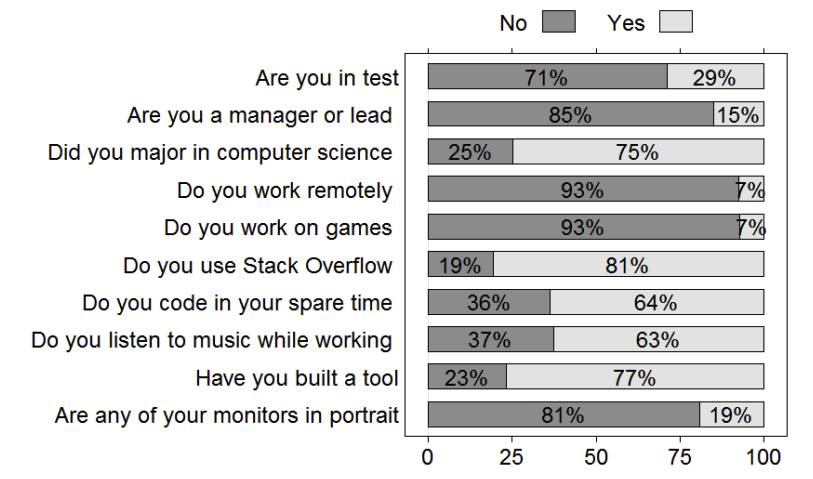
\includegraphics[width=\textwidth]{demographics.png}
        \caption{Distribution of demographic and work-practice responses.}
        \label{fig:demographics}
    \end{subfigure}
    \hfill
    \begin{subfigure}{0.45\textwidth}
        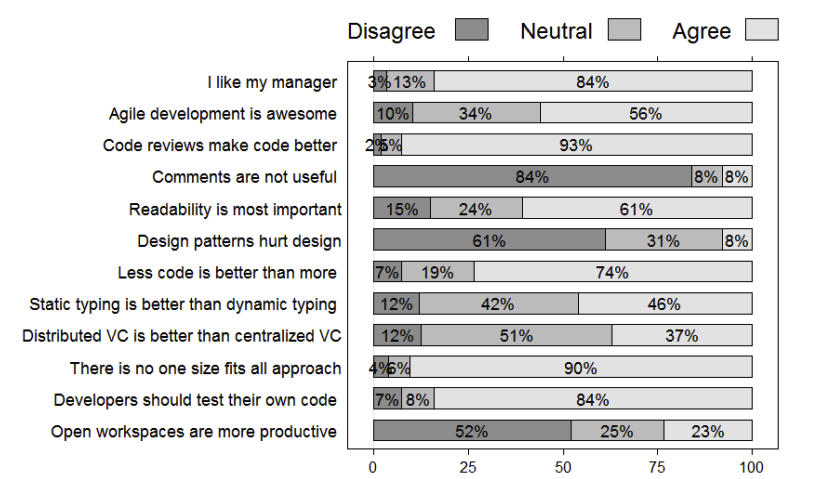
\includegraphics[width=\textwidth]{developer.png}
        \caption{Distribution of beliefs about development practices.}
        \label{fig:developer_beleifs}
    \end{subfigure}
    \caption{Survey response distributions}
\end{figure}

\paragraph{Distribution of Beliefs and Work Practices}
The survey results indicate substantial agreement among engineers on several core development practices, alongside clear disagreement on others {Figure \ref{fig:demographics}}. A majority of respondents agreed that developers should test their own code, that code reviews and comments enhance code quality, and that readability is a central attribute of well-written software. Similarly, more than half endorsed the view that less code is preferable to more code.

In contrast, certain topics generated limited consensus (Figure \ref{fig:developer_beleifs}). Opinions regarding static versus dynamic typing and distributed versus centralized version control systems were widely dispersed, with a large proportion of neutral responses. The question of open workspaces proved particularly controversial, with a majority rejecting the claim that they improve productivity, while a notable minority supported it.

\paragraph{Limited Personality Differences Across Roles}
One of the most notable findings is the absence of significant personality differences between developers (SDEs) and testers (SDETs). This suggests that role assignment within the organization does not strongly correspond to differences in core personality traits as measured by the Five-Factor Model.

However, differences were observed for leadership roles. Managers and leads exhibited higher levels of conscientiousness and extraversion compared to non-managers. This pattern indicates that leadership positions may be associated with greater organizational discipline, reliability, and sociability.

\paragraph{Personality and Work Practices}
The analysis identified statistically significant relationships between personality traits and specific work practices. Engineers who reported listening to music while working were generally more open and extraverted and slightly less conscientious.

More substantial differences were observed among engineers who had built tools on their own initiative. These individuals scored higher in openness, conscientiousness, and extraversion, and lower in neuroticism compared to those who had not built such tools. This pattern suggests that proactive technical initiative may be associated with cognitive flexibility, organizational reliability, social engagement, and emotional stability.

\paragraph{Personality and Professional Beliefs}
Personality traits were also associated with specific professional beliefs. The clearest example concerns attitudes toward Agile development. Engineers who agreed with the statement “Agile development is awesome” scored higher on extraversion and lower on neuroticism compared to those who disagreed.

Additionally, openness was positively associated with agreement that distributed version control systems are preferable to centralized systems. These results suggest that personality traits may shape how engineers evaluate development methodologies, collaboration structures, and tooling philosophies.

\paragraph{Robustness After Multiple Hypothesis Testing}
Initial statistical testing identified 20 significant personality differences at the $p < 0.05$ level. However, after applying the Benjamini–Hochberg correction to control the false discovery rate, only 6 differences remained statistically significant. This adjustment underscores the importance of accounting for multiple hypothesis testing and indicates that, although certain personality associations exist, the overall magnitude of differences is limited.

The reduction in statistically significant findings reinforces the broader conclusion that personality differences within the engineering population are present but not pervasive.

\subsection{Threats to Validity}
The primary threat to validity arises from the study’s confinement to a single large industrial organization. Although the organization exhibits substantial internal diversity in terms of engineering practices and employee backgrounds, the findings may not generalize to smaller companies, startups, or open-source communities. Additionally, the survey was explicitly framed as a “Developer Personality Survey,” which introduces the possibility of self-selection bias; individuals with an interest in personality assessment may have been more inclined to participate. This could systematically influence the distribution of personality traits within the respondent sample. Furthermore, as with any self-reported survey, responses may be affected by social desirability bias or subjective interpretation of survey items, potentially influencing both reported beliefs and personality measures.

\section{Implications}
\paragraph{Limited Role of Personality Testing in Hiring}
The findings suggest that personality differences among software engineers are relatively limited in scope. Given the small number of statistically significant differences observed, the results imply that the role of personality testing in hiring decisions may be less influential than sometimes assumed. However, the study does not draw definitive conclusions on this matter and emphasizes that additional research—particularly regarding the social dynamics of engineering teams—is necessary before making strong claims about the utility of personality assessments in recruitment or selection processes.

\paragraph{Absence of Expected Differences}
An important implication arises from the absence of personality differences in areas where such distinctions might have been anticipated. No significant differences were observed between developers and testers, nor for engineers working remotely versus locally, working on games, or holding particular views about open workspaces or typing paradigms. This suggests that common assumptions about personality-based distinctions across roles or preferences may not be strongly supported in this industrial context.

\paragraph{Opportunities for Future Research}
The study highlights broader opportunities for continued investigation into personality within software engineering teams. In particular, it underscores the need for further research on how personality interacts with collaborative environments, team structures, and organizational contexts. Additionally, the authors emphasize the value of systematically polling engineers about their workplace practices and beliefs, indicating that large-scale empirical surveys can provide foundational statistics and open new avenues for understanding human factors in software engineering.
